%% -*- coding: utf-8 -*-
\documentclass[12pt,pagesize,paper=landscape,paper=192mm:108mm]{scrbook} 
%1920x1080 1280x720
\areaset[current]{192mm}{108mm}
\usepackage{calc}
\usepackage[T2A]{fontenc}
\usepackage[utf8]{inputenc}
\usepackage[english,russian]{babel}
\usepackage{microtype}
\usepackage{misccorr}
\usepackage{cmap}
%\usepackage[unicode=true]{hyperref}
\usepackage{graphicx}
\usepackage{amssymb}
\usepackage{amsmath}
%\usepackage{srcltx}
\usepackage{textcomp}
\usepackage{xspace}
\usepackage{calc}
%научные символы и смайлики \smiley \frownie
\usepackage{wasysym}
\usepackage{ccicons}
\begin{document}
\begin{titlepage}
  \vspace*{-0.5em}
  \begin{center}    
    \hspace*{3em}
    \begin{minipage}[t]{3em}
      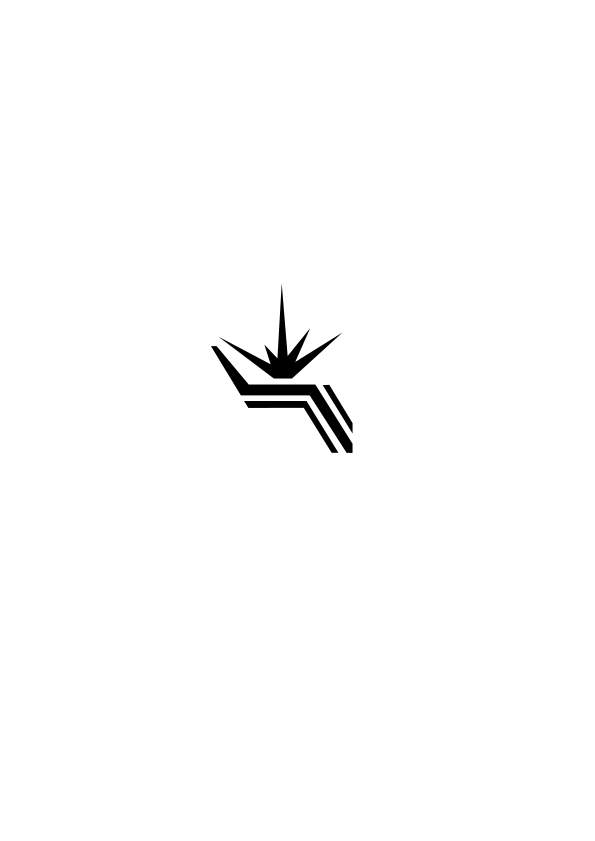
\includegraphics[width=\textwidth]{../BINP-logo}
    \end{minipage}\hfill
    \begin{minipage}{0.23\linewidth}
    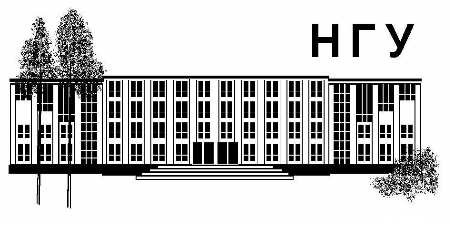
\includegraphics[width=\textwidth]{../NSU-logo}
    \end{minipage}
    \hfill
    \hspace*{6em}


    Кафедра теоретической физики физического факультета НГУ
    \medskip

    \Large
    Профессор Черняк В.\,Л.
    \bigskip

    \huge
    \textbf{Теория электрослабых взаимодействий}
    \bigskip

    \Large
    Лекция № 1
    \vfill

    % \normalsize
    % \begin{minipage}{0.65\linewidth}
    % \end{minipage}
    \vfill

\normalsize    Новосибирск 2013
  \smallskip

  \ccbysa
  \end{center}
\end{titlepage}
\newpage

\vspace*{-1em}
\begin{center}
 \vfill
  \begin{minipage}{0.66\linewidth}
    Вводная лекция. Иерархия времён сильных, электромагнитных и слабых
    распадов. Основная цель курса "--- слабые распады преимущественно в
    борновском приближении, Стандартная модель в~целом.  Общее
    напоминание про КХД. Лагранжиан КХД. Симметрии лагранжиана
    КХД. Калибровочная симметрия. Внешние симметрии: флейворная
    симметрия $SU(N_F)$. Правые и левые
    спиноры.  Киральность и спиральность. Киральная симметрия
    $SU(N_F)_L\otimes SU(N_F)_R$ для
    безмассовых кварков.  Иерархия по реальным массам кварков и
    лептонов. Изотопическая симметрия сильного взаимодействия.
    Точность изотопической симметрии. Симметрии лагранжианов и
    вакуумных состояний: отличие КЭД и КХД.  Спонтанное нарушение
    симметрии. Динамические массы кварков и связь непертурбативных
    эффектов с точностью изотопической симметрии.
  \end{minipage}
  \vfill
  % Новосибирск 2013

  % \normalsize \ccbysa
\end{center}
\end{document}
